%%
%% Copyright 2007, 2008, 2009 Elsevier Ltd
%%
%% This file is part of the 'Elsarticle Bundle'.
%% ---------------------------------------------
%%
%% It may be distributed under the conditions of the LaTeX Project Public
%% License, either version 1.2 of this license or (at your option) any
%% later version.  The latest version of this license is in
%%    http://www.latex-project.org/lppl.txt
%% and version 1.2 or later is part of all distributions of LaTeX
%% version 1999/12/01 or later.
%%
%% The list of all files belonging to the 'Elsarticle Bundle' is
%% given in the file `manifest.txt'.
%%

%% Template article for Elsevier's document class `elsarticle'
%% with numbered style bibliographic references
%% SP 2008/03/01
%%
%%
%%
%% $Id: elsarticle-template-num.tex 4 2009-10-24 08:22:58Z rishi $
%%
%%
\documentclass[preprint,12pt,3p]{elsarticle}

%\documentclass[final,3p,times]{elsarticle}
%% Use the option review to obtain double line spacing
%% \documentclass[preprint,review,12pt]{elsarticle}

%% Use the options 1p,twocolumn; 3p; 3p,twocolumn; 5p; or 5p,twocolumn
%% for a journal layout:
%% \documentclass[final,1p,times]{elsarticle}
%% \documentclass[final,1p,times,twocolumn]{elsarticle}
%% \documentclass[final,3p,times]{elsarticle}
%% \documentclass[final,3p,times,twocolumn]{elsarticle}
%% \documentclass[final,5p,times]{elsarticle}
%% \documentclass[final,5p,times,twocolumn]{elsarticle}

%% if you use PostScript figures in your article
%% use the graphics package for simple commands
%% \usepackage{graphics}
%% or use the graphicx package for more complicated commands
%% \usepackage{graphicx}
%% or use the epsfig package if you prefer to use the old commands
%% \usepackage{epsfig}

%% The amssymb package provides various useful mathematical symbols
\usepackage{amssymb}
\usepackage{graphicx}
\usepackage[utf8]{inputenc}
\usepackage{color}
\usepackage[procnames]{listings}


\graphicspath{ {img/} }
%% The amsthm package provides extended theorem environments
%% \usepackage{amsthm}

%% The lineno packages adds line numbers. Start line numbering with
%% \begin{linenumbers}, end it with \end{linenumbers}. Or switch it on
%% for the whole article with \linenumbers after \end{frontmatter}.
%% \usepackage{lineno}

%% natbib.sty is loaded by default. However, natbib options can be
%% provided with \biboptions{...} command. Following options are
%% valid:

%%   round  -  round parentheses are used (default)
%%   square -  square brackets are used   [option]
%%   curly  -  curly braces are used      {option}
%%   angle  -  angle brackets are used    <option>
%%   semicolon  -  multiple citations separated by semi-colon
%%   colon  - same as semicolon, an earlier confusion
%%   comma  -  separated by comma
%%   numbers-  selects numerical citations
%%   super  -  numerical citations as superscripts
%%   sort   -  sorts multiple citations according to order in ref. list
%%   sort&compress   -  like sort, but also compresses numerical citations
%%   compress - compresses without sorting
%%
%% \biboptions{comma,round}

% \biboptions{}


\begin{document}

\begin{frontmatter}

\title{Assignment 1: Mixnets}

\author{Santiago Aragón}
\address{s.e.aragonramirez@student.utwente.nl}

\author{Owais Ahmed}
\address{o.ahmed@student.utwente.nl}
\address{University of Twente}

%\begin{abstract}
%Text of abstract. Text of abstract. %Text of abstract. Text of abstract. %Text of abstract.
%\end{abstract}


\end{frontmatter}

%%
%% Start line numbering here if you want
%%
% \linenumbers

%% main text



\section*{Assignment 1}
\textbf{Part A:}
We wrote the script showed in Appendix A to interact with the mixnet i.e., turn on/off the mixnet, send messages, process the logs and perform an \textit{n\-1} attack.
\newline

\textbf{Part B:}
We sent a message to TIM using the \textit{send\_message} method as shown below in Appendix A.
\begin{verbatim}send_message('TIM     ','s1750542  and  s1736574') \end{verbatim}

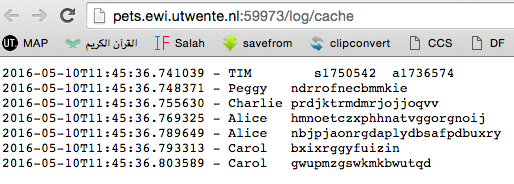
\includegraphics[width=\textwidth]{tim}

\textbf{Part C:}

\begin{figure}[h]
\caption{Frequency of messages received against time in the same second.}
\centering
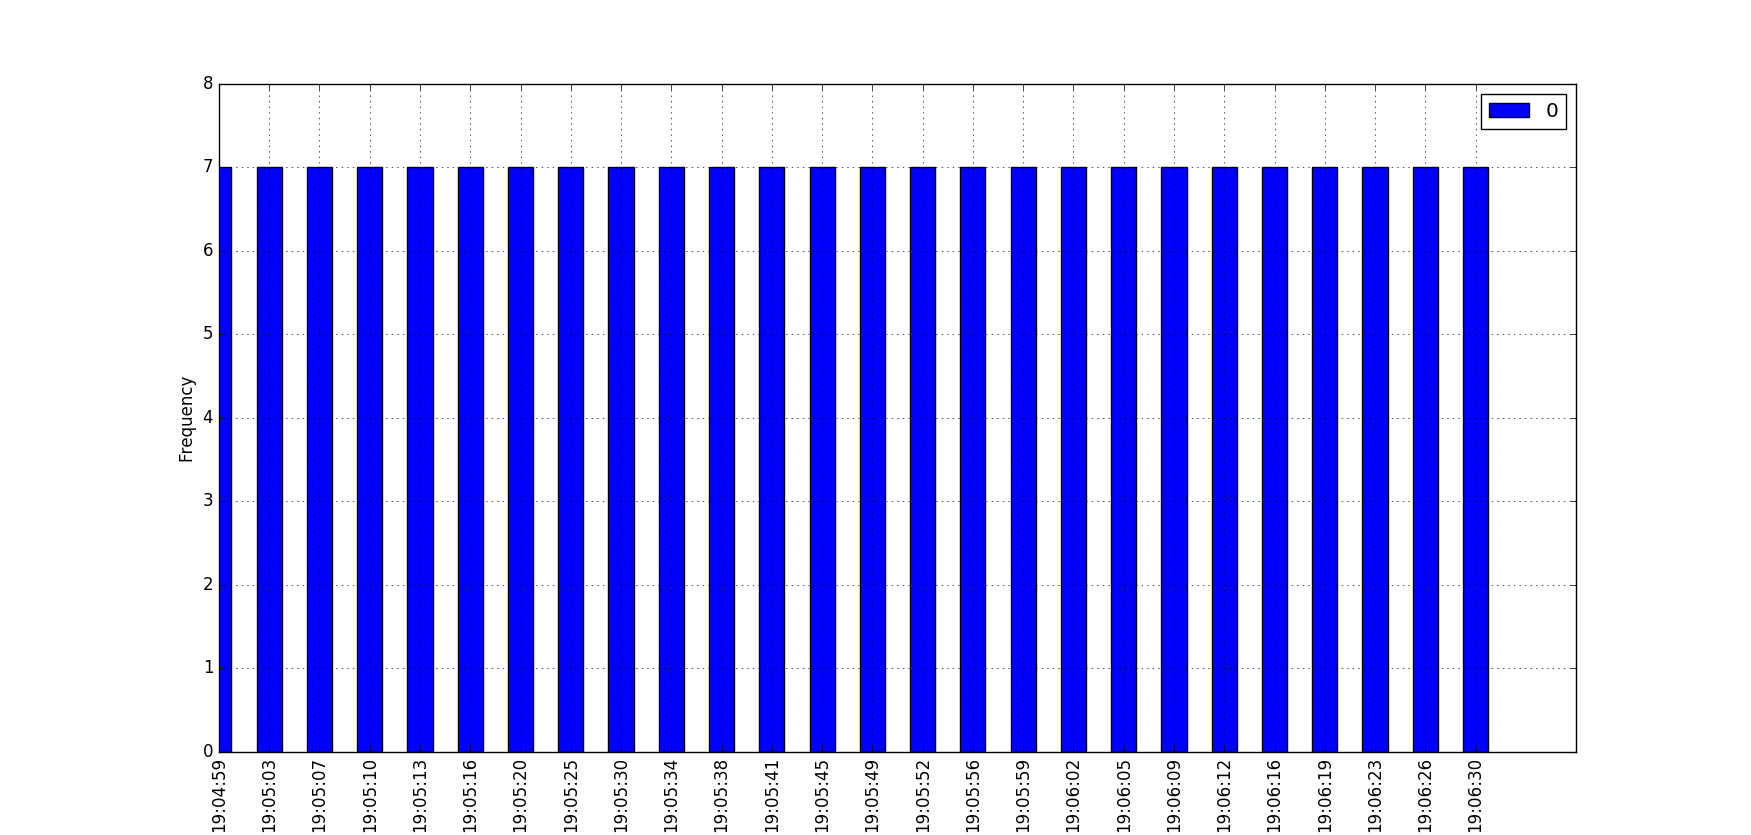
\includegraphics[width=\textwidth]{one_c}
\end{figure}

We parsed the cache log to analyse the individual messages and performed frequency analysis as shown in Figure: 1 by counting the number of messages received in a particular second and plotted the results in a bar chart graph. We observed that mostly seven messages were received in the cache log in a particular second, however in certain instances, the average of consecutive messages received in two seconds was seven. We therefore came to the conclusion that $n_C$ is 7, and since we know that the threshold of $n_A$ = $n_B$ = $n_C$, it implies that $n_A$ , $n_B$ and $n_C$ is 7.

\section*{Assignment 2}
\textbf{Part A:}
\newline

We sent individual messages one by one with a short time delay and observed the output via the cache log by parsing the message fields. We observed that the messages forwarded by MIX C to the CACHE NODE had a frequency of mostly 6 or 9. We learned that the sum of messages received in consecutive seconds was always a factor of 3, as shown in Figure: 2. We therefore, we came to the conclusion that the threshold of $n_C$ is 3.
\newline
\begin{figure}[h]
\caption{Frequency of messages received against time in the same second.}
\centering
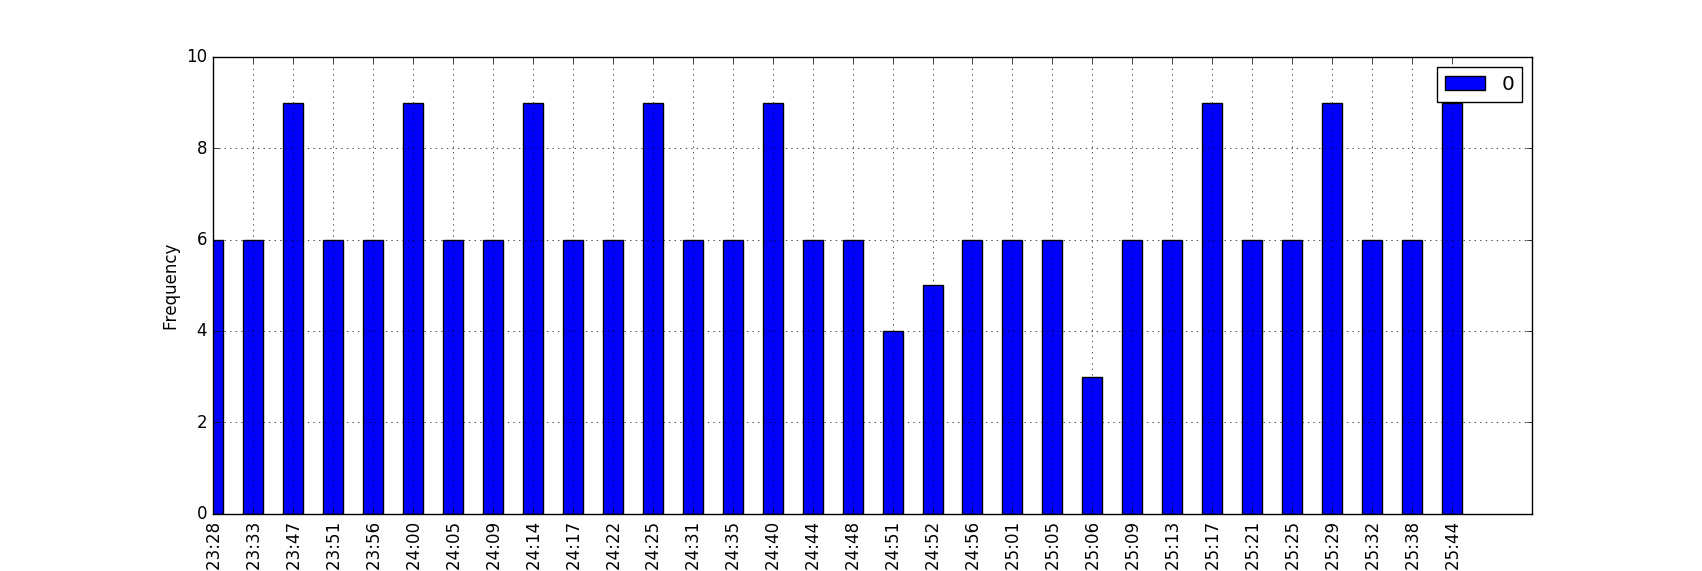
\includegraphics[width=\textwidth]{second}
\end{figure}
\newline
We kept a count of the messages entering the second mixnet via MIX A and the messages received in the cache log after reaching the threshold $n_C$. After the first 8 messages passed through MIX A, only 6 messages were displayed in the cache log. Since we know that the threshold of MIX B has to be at least more than $2n_C$ and less than $3n_C$. This implies that the threshold of MIX B is 6 $<$ $n_B$ $<$ 9. Furthermore, we have only inject 8 messages and we know that $n_A\geq 1$ , therefore we conclude that the threshold $n_B$ is 7.
\newline
We kept a count of the messages entering the second mixnet via MIX A and the messages received in the cache log after reaching the threshold $n_C$. After the first 8 messages passed through MIX A, only 6 messages were displayed in the cache log, that denotes that 1 $\leq$ $n_A, n_B$ $\leq$ 8. We sent more messages one by one until a second batch of 6 messages were received in the cache log. We noted that after sending 6 more messages, another batch of 6 messages was received in the cache log, this further helped us to analyse that MIX A always accepted even number of messages and the least common factor of the input messages to obtain an output was always 2. We therefore concluded that the threshold of $n_A$ is 2.

\begin{center}
Threshold of $n_A$ is 2

Threshold of $n_B$ is 7

Threshold of $n_C$ is 3
\end{center}




\textbf{Part B:}

\section*{Assignment 3}
\textbf{Part A:}

To deanonymize the party that is communicating with TIM we launch a n-1 attack. We recall that we are a global active attacker with insert capabilities, namely, we have access to two logs one at the entrance (client log) of the mixnet and one at very end (cache log).

We have find the threshold of every MIX in section~\ref{sec2} and we know that the first 2 batches are triggered with 8 messages. Thus, after starting the mixnet we insert 7 messages and wait for a message coming from some mixnet user. The very first message that arrive will push 6 messages to the cache, to which we have access through the logs. By comparing the client log and the cache log we are able to deanonymize the first message that enters the mixnet after our first 7 messages. We define a function called \textit{n\_1\_attack} where we start the mixnet, perform a n-1 attack and repeats until the deanonymized user is the one that communicates with Tim. \newline

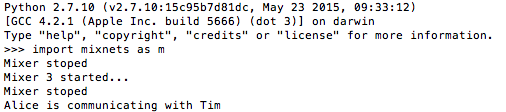
\includegraphics[width=\textwidth]{alice}

\textbf{Part B:}
The first method is to prevent less than 3 users in one particular batch of messages to be flushed to the next mix node after reaching its threshold.
The second way of preventing such type of attacks is by randomising the threshold of each node after every few random time delays. This will prevent the attacker to perform n-1 attack.





%% appendix sections are then done as normal sections
\appendix
\section{Appendix}



% \section{Mixnet 1}
% \section{Mixnet 2}
% \section{Mixnet 3}

\section{Mixnet 1}

\section{Mixnet 3}
\begin{lstlisting}[language=Python]
# -*- coding: utf-8 -*-
import urllib2
import socket
import struct
from Crypto.PublicKey import RSA
from Crypto import Random
from Crypto.Cipher import PKCS1_OAEP
from Crypto.Cipher import AES
from Crypto.Protocol.KDF import PBKDF2
import random
import string
from datetime import datetime

import numpy as np
import matplotlib.mlab as mlab
import matplotlib.pyplot as plt
import pandas
from collections import Counter
from time import sleep


def pack_message(message):
    key_cache = 'keys/public_key_Cache.pem'
    key_c = 'keys/public_key_C.pem'
    key_b = 'keys/public_key_B.pem'
    key_a = 'keys/public_key_A.pem'
    e1 = create_message(key_cache, message)
    e2 = create_message(key_c, e1)
    e3 = create_message(key_b, e2)
    e4 = create_message(key_a, e3)
    return e4


#  Cache encyption
def create_message(key_path, message):
    key_rsa = open(key_path, 'rb').read()
    k_aes, iv = generate_key_iv()
    msg = '%s%s' % (k_aes, iv)
    e1_rsa = rsa_encrypt(key_rsa, msg)
    e1_aes = aes_encrypt(k_aes, iv, message)
    e1 = '%s%s' % (e1_rsa, e1_aes)
    return e1


def generate_not_random_key_iv():
    N = 5
    key_size = 16
    iterations = 1
    key = b'J6EXO'
    salt = b'??K7|3??PP?x?'
    iv = b'a'*16
    derived_key = PBKDF2(key, salt, key_size, iterations)

    return derived_key, iv


def generate_key_iv():
    N = 5
    key_size = 16  # AES128
    iterations = 1000
    key = b''.join(random.SystemRandom().choice(string.ascii_uppercase + string.digits) for _ in range(N))
    salt = Random.new().read(key_size)

    iv = Random.new().read(AES.block_size)
    derived_key = PBKDF2(key, salt, key_size, iterations)

    return derived_key, iv


def rsa_encrypt(key, message):
    keyPub = RSA.importKey(key)
    cipher = PKCS1_OAEP.new(keyPub)
    ciphertext = cipher.encrypt(message)
    return ciphertext


def aes_encrypt(key, iv, message):
    # key_size = 32 #AES256
    # iterations = 10000
    # key = b'password'
    BS = 16
    add_padding = lambda s: s + (BS - len(s) % BS) * chr(BS - len(s) % BS)
    p_msg = add_padding(message)
    cipher = AES.new(key, AES.MODE_CBC, iv)
    return cipher.encrypt(p_msg)



def recv_one_message(sock):
    lengthbuf = recvall(sock, 4)
    length, = struct.unpack('!I', lengthbuf)
    return recvall(sock, length)


def recvall(sock, count):
    buf = b''
    while count:
        newbuf = sock.recv(count)
        if not newbuf:
            return None
        buf += newbuf
        count -= len(newbuf)
    return buf


def send_one_message(sock, data):
    length = len(data)
    sock.sendall(struct.pack('!I', length))
    sock.sendall(data)

def message_num():
    log = parseClientLog()
    times = list()

    if log is not None and log != '':
        for entry in log.split('\n'):
            if entry != '':
                times.append(parse_entry(entry)['date'].strftime('%H:%M:%S'))
    return len(times)


def cache_num():
    log = parseCacheLog()
    times = list()

    if log is not None and log != '':
        for entry in log.split('\n'):
            if entry != '':
                times.append(parse_entry(entry)['date'].strftime('%H:%M:%S'))
    return len(times)


def parseClientLog():
    log_add = 'http://pets.ewi.utwente.nl:59973/log/clients'
    try:
        log = urllib2.urlopen(log_add).read()
        if log == '':
            print 'Empty log...'
            pass
        return log
    except Exception, e:
        print 'No log found '
        return ''


def parseCacheLog():
    log_add = 'http://pets.ewi.utwente.nl:59973/log/cache'
    try:
        log = urllib2.urlopen(log_add).read()
        if log == '':
            print 'Empty log...'
            pass
        return log
    except Exception, e:
        print 'No log found '
        return None


def start(mix_num):
    stop()
    log_add = 'http://pets.ewi.utwente.nl:59973/cmd/mix%s' % mix_num
    urllib2.urlopen(log_add)
    print 'Mixer %s started...' % mix_num


def stop():
    log_add = 'http://pets.ewi.utwente.nl:59973/cmd/reset'
    urllib2.urlopen(log_add)
    sleep(2)
    print 'Mixer stoped'


def parse_entry(entry):
    e =  entry.split(' ')
    date = datetime.strptime(e[0],"%Y-%m-%dT%H:%M:%S.%f")
    participant = e[2]
    message = e[3]
    return {'date': date, 'participant': participant, 'message': message}


def second_freq(log):
    times = list()
    if log is not None and log != '':
        for entry in log.split('\n'):
            if entry != '':
                times.append(parse_entry(entry)['date'].strftime('%H:%M:%S'))

        counts = Counter(times)
        df = pandas.DataFrame.from_dict(counts, orient='index')
        df =  df.sort_index()
        df.plot(kind='bar')
        plt.xlabel('Time')
        plt.ylabel('Frequency')
        plt.axis([0, len(counts)+1, 0, max(counts.values())+1])
        plt.grid(True)
        plt.show()


def send_message(recipient, message):
    message = '%s\t%s' % (recipient, message)
    HOST = 'pets.ewi.utwente.nl'
    PORT = 51666
    clientsocket = socket.socket(socket.AF_INET, socket.SOCK_STREAM)
    clientsocket.connect((HOST, PORT))
    e4 = pack_message(message)
    send_one_message(clientsocket, e4)


def check_for_tim():
    log = parseCacheLog()
    if log is not None and log != '':
        for entry in log.split('\n'):
            if entry != '':
                e = parse_entry(entry)
                if e['participant'] == 'Tim':
                    return True
    return False

def one_a():
    start(1)
    # sleep(3)
    send_message('OWAIS','That is not secret message')
    sleep(10)
    stop()

def one_b():
    start(1)
    send_message('TIM     ','s1750542  a1736574')
    sleep(10)
    stop()

def one_c():
    start(1)
    for x in range(120):
        send_message('ME ', 'message #%s'% ( x))
        print 'injecting message #%s\r' % ( x),
    second_freq(parseCacheLog())
    stop()

def first_client():
    log = parseClientLog()
    e = parse_entry(log.split('\n')[0])['participant']
    # print parse_entry(log.split('\n')[0])
    return e



def not_me():
    log = parseCacheLog()
    if log is not None and log != '':
        for entry in log.split('\n'):
            if entry != '':
                e = parse_entry(entry)
                if e['participant'] != 'ME':
                    return e['participant']

def n_1_a():
    start(3)
    sleep(.05)
    send_message('ME ', '-'*7)
    send_message('ME ', '-'*7)
    send_message('ME ', '-'*7)
    send_message('ME ', '-'*7)
    send_message('ME ', '-'*7)
    send_message('ME ', '-'*7)
    send_message('ME ', '-'*7)
    log = parseClientLog()
    if log == '':
        message_sent = 7
        while cache_num() < 6:
            pass
        stop()
        sleep(2)
        if not check_for_tim() and not_me() is not  None:
            rec = not_me()
            sen = first_client()
            print '%s is communicating with %s' %(sen, rec)
            n_1_a()
        elif not_me() is  None:
            n_1_a()
        else:
            rec = not_me()
            sen = first_client()
            print '%s is communicating with %s' %(sen,rec)
    else:
        n_1_a()



n_1_a()

\end{lstlisting}


\label{appendix-sec1}
%% References
%%
%% Following citation commands can be used in the body text:
%% Usage of \cite is as follows:
%%   \cite{key}         ==>>  [#]
%%   \cite[chap. 2]{key} ==>> [#, chap. 2]
%%
%% References with bibTeX database:

% \bibliographystyle{elsarticle-num}
% % \bibliographystyle{elsarticle-harv}
% % \bibliographystyle{elsarticle-num-names}
% % \bibliographystyle{model1a-num-names}
% % \bibliographystyle{model1b-num-names}
% % \bibliographystyle{model1c-num-names}
% % \bibliographystyle{model1-num-names}
% % \bibliographystyle{model2-names}
% % \bibliographystyle{model3a-num-names}
% % \bibliographystyle{model3-num-names}
% % \bibliographystyle{model4-names}
% % \bibliographystyle{model5-names}
% % \bibliographystyle{model6-num-names}
% \bibliography{sample}


\end{document}

%%
%% End of file `elsarticle-template-num.tex'.
